\documentclass[12pt]{article}
\usepackage[utf8]{inputenc}
\usepackage{blindtext}
\usepackage{amsmath}
\usepackage{graphicx}
\usepackage{array}
\graphicspath{ {./images/} }

\begin{document}
\begin{titlepage}
\begin{center}
    \LARGE\textbf{{Utility-Runtime Trade-Off Analysis in Queue-Density Estimation}}\\
    \vspace{5cm}
   
   
    \hrule
     \vspace{1cm}
    \large{BY}\\
      \vspace{0.15cm}
    \Large\textbf{{KURISETI RAVI SRI TEJA - 2019CS10369}}\\
    \Large\textbf{{GATTU KARTHIK - 2019CS10348}}\\
      \vspace{1cm}
    \hrule
    
\end{center}


\end{titlepage}
\tableofcontents

\newpage
\section{Introduction}
\subsection{Traffic Densities and their Calculations}
\subsubsection{Queue Density}
\paragraph{}
  Queue Density is defined as the fraction of the area of the road that is occupied by the vehicles.It's value lies in the range [0,1].For calculating the queue density of a particular road, we first transform the frame i.e., perform perspective correction using homography to make the road parallel to the plane of paper and then crop the unnecessary portion. The obtained matrix is associated a name frame f.  The same operation is performed to a reference image which contains no traffic(i.e., empty roads) and the obtained frame is given a name frame ref. We associate a quantity \textbf{required cells} for each frame.It is defined as the number of cells in frame f such that absolute difference in pixels between frame f and frame ref is less than 30.Then queue density is calculated by the formula.
   \[\text{Queue Density}=\frac{\text{Required cells}} {\text{Total no.of cells in frame f}}\]
   
 \vspace{5mm}
   
\subsubsection{Dynamic Density}
\paragraph{}
  Dynamic Density is defined as the fraction of the area of the road that is occupied by the moving vehicles.It's value lies in the range [0,1].For calculating dynamic densities usually optical flow algorithms are used which are very complex and gives accurate results.For calculating dynamic density,we used highly approximate techniques i.e., we found difference between every two successive frames and counted the no.of cells whose pixel values are more than 5 after applying homography and cropping the image.
   \[\text{Dynamic Density}=\frac{\text{Number of cells with pixel value $>$ 10}} {\text{Total no.of cells in frame f}}\]

\newpage

\section{Metrics}
 \subsection{Baseline for Metrics}
 We will consider the outputs produced when we are processing the whole video frame-by frame as the baseline.
 
\subsection{Runtime Metrics}
 For measuring the runtime of program, we used the built in clock provided by the std::chrono library which can be used to calculate the time taken for execution of the program in milliseconds which depends on the way video will be processed.
 
 \subsection{Utility Metrics}
 We used the mean of squares of difference of queue-density value obtained in each method used and corresponding queue-density in baseline as absolute  error value and took utility as (1-relative error)*100  for plotting various graphs where relative error was taken as 
  \[\text{Relative Error}=\frac{\text{Absolute Error}} {\text{Average Queue Density of all frames in the video}}\].
 
 \section{Various Methods for Trade-Off Analysis}
 \subsection{Sub-Sampling Frames}
 In this process we would process every kth frame starting from 1st frame.
 The baseline for this method is to process every frame.
 We tested this process with the values of k as 2,5,10,50,100,500.
 
 \subsection{Changing Resolutions}
 In this process we would use the standard resolutions which are lower than the resolution of given video i.e., 960*540,480*270,240*135,120*67,60*33 and compare them with 1920*1080 resolution(original image).
 
 \newpage
 
 \subsection{Using pthreads}
  For improving the speed of execution we used the pthreads provided by the OS.
  We tried to speed up the execution in two possible ways.
  
 \subsubsection{Processing Consecutive frames using different threads }
 In this process we created multiple threads and used them to process consecutive frames in such a way that each frame is processed by only one thread.
 
% \subsubsection{Processing each frame with different threads }
% In this process multiple threads were used to process each frame i.e., part of each frame was processed by a thread.


\section{Utility-Runtime Plots}
All the data used here was produced using Mac-Book Air laptop with 1.6GHz dual-core Intel Core i5, Turbo Boost up to 3.6GHz, with 4MB L3 cache.
\subsection{Sub-Sampling Frames}
\large{\textbf{k} is the parameter by which we skipped frames.}

\begin{center}
\begin{tabular}{|m{10 em}|m {10 em} | m {10 em}|} 
 \hline
 \textbf{Value of k} & \textbf{Runtime in seconds} & \textbf{Utility Value}\\ 
 &  & \textit{(utility-99.95)*10000}\\[1.5 ex]
 \hline\hline
 2 & 122.337 & 449.408  \\ 
 \hline
 5 & 68.520 & 419.045  \\
 \hline
 10 & 49.715 & 408.909  \\
 \hline
 50 & 33.548 & 400.806 \\
 \hline
 100 & 30.383 & 399.799 \\
 \hline
 500 & 30.740 & 398.997  \\ [1ex] 
 \hline
\end{tabular}
\end{center}
\newpage
\Large\textbf{{Corresponding Plots:}}
\begin{center}
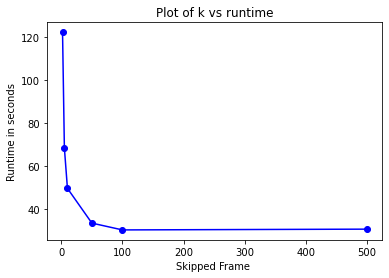
\includegraphics[scale=0.9] {sub-sampling/k vs runtime.png} \\
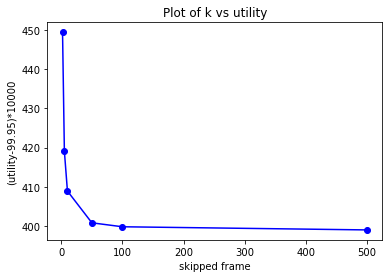
\includegraphics[scale=0.9] {sub-sampling/k vs utility.png} \\

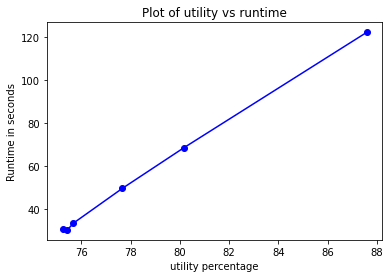
\includegraphics[scale=0.9] {sub-sampling/utility vs runtime.png} 
\end{center}

\subsection{Resolution Change}
\large{\textbf{X,Y} are dimensions of image to which we are compressing  or expanding  by changing resolution is the parameter by which we skipped frames.}
 
 \begin{center}
 \begin{tabular}{|m{6 em}|m {6 em}|m {7 em}| m {10 em}|} 
 \hline
 \textbf{Value of X} & \textbf{Value of Y} & \textbf{Value of XY} &\textbf{Value of log(XY)}\\ 
 
 \hline\hline
 60 & 33 & 1980  & 7.591  \\ 
 \hline
 120 & 67 & 8040  & 8.992 \\
 \hline
 240 & 135 & 32400  & 10.386 \\
 \hline
 480 & 270 & 129600 & 11.772 \\
 \hline
 960 & 540 & 518400  & 13.159 \\
 \hline
 1920 & 1080 & 2073600  & 14.545 \\ [1ex] 
 \hline
\end{tabular}
\end{center}

%196.950075, 199.38872899999998, 201.61550699999998, 211.288206, 247.88394, 421.86749%

\begin{center}
 \begin{tabular}{|m{9 em}|m {10 em}|m {11 em}|} 
 \hline
 \textbf{Value  of log(XY)} & \textbf{Runtime in seconds} & \textbf{Utility Value}\\ 
 &  & \textit{(utility-99.999)*100000}\\[1.5 ex]
 \hline\hline
 7.591 & 196.950 & 99.830  \\ 
 \hline
 8.992 & 199.389 & 99.937  \\
 \hline
 10.386 & 201.616 & 99.965  \\
 \hline
 11.772 & 211.288 & 99.964 \\
 \hline
 13.159 & 247.884 & 99.970 \\
 \hline
 14.545 & 421.867 & 99.971  \\ [1ex] 
 \hline
\end{tabular}
\end{center}

\Large\textbf{{Corresponding Plots:}}
\begin{center}
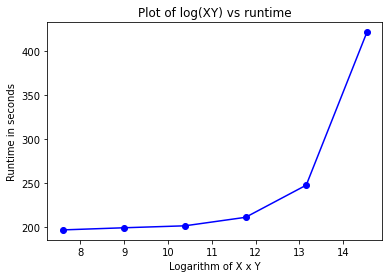
\includegraphics[scale=0.9] {resolution/xy vs runtime.png} 
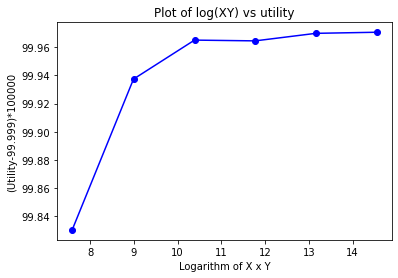
\includegraphics[scale=0.9] {resolution/xy vs utility.png} 
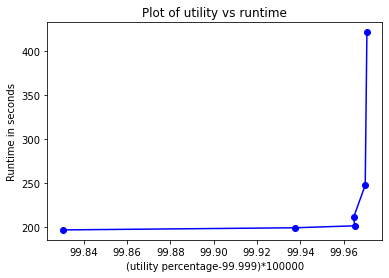
\includegraphics[scale=0.9] {resolution/utility vs runtime.png} 
\end{center}

 
\subsection{Using pthreads}
\subsubsection{Using distinct threads for consecutive frames}
\large{\textbf{n}  is the number of threads used.In this case utility is redundant as its value will be 100.}
 
 \begin{center}
 \begin{tabular}{|m{7 em}|m {10 em}|m {10 em}|} 
 \hline
 \textbf{Value of n} & \textbf{Runtime in seconds} & \textbf{Utility}\\ 
 
 %183.288793, 182.028051, 181.227609, 187.827055%
 \hline\hline
 1\textbf{(Base-Case)}& 194.334 & 100.0  \\
  
 \hline
 2 & 183.289 & 100.0  \\
 \hline
 3 & 182.028 & 100.0  \\
 \hline
 4 & 181.228 & 100.0  \\
 \hline
 5 & 187.827 & 100.0 \\ [1ex] 
 \hline
\end{tabular}
\end{center}

 \Large\textbf{{Corresponding Plots:}}
 \begin{center}
 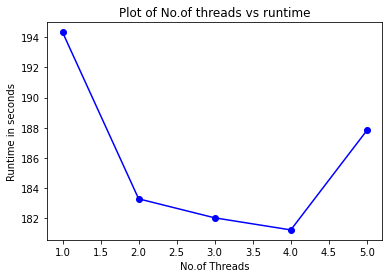
\includegraphics[scale=0.9] {alternateframes/threads vs runtime.png} 
 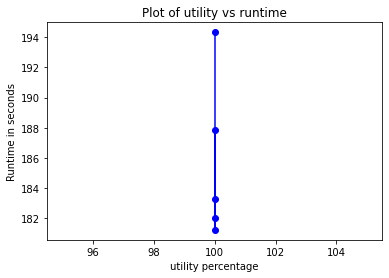
\includegraphics[scale=0.9] {alternateframes/utility vs runtime.png} 
 \end{center}
\newpage

 \section{Conclusions}
 \begin{itemize}
\normalsize{

\item When we are using pthreads to process consecutive frames,we see that the runtime doesn't change much with the number of threads used.This might be due to the fact that the time taken for creating the thread could be almost same as the time taken by that thread to process the frames.

\item We see that decreasing resolution has negligible effect on utility i.e., the error value is less than 0.01\% but we see that the runtime is very less with smaller resolutions frames although it takes some time for creating new frames from older frames it is very small(3-4 seconds).

\item We see that utility increases with runtime in all cases(except in threads case where error is obviously \textbf{zero}) which is evident as for minimizing the error value we need to make more number of computations thereby increasing the runtime.

\item We can use mixture of above methods i.e., we can reduce resolution of images and use multiple threads for reducing runtime and with utility of around 99.999\% as multiple threads have no effect on utility values.

\item When we use multiple threads,it increases the CPU Temperature and so using multiple pthreads is not preferred for embedded systems used in hot conditions.
}
 
\end{itemize}

\section{References:}
\begin{enumerate}
   \normalsize{
    \item https://docs.opencv.org/master/
    \item https://learnopencv.com/
    }
\end{enumerate}
\end{document}
